\section{Eprobung des Reglers an der Regelstrecke}\label{section_corner_balance_test}
Der nächste Schritt besteht darin die Ergebnisse der letzten Abschnitte an der Regelstrecke zu erproben, wozu der in der Simulation optimierte Regler verwendet wird. Dieser führt zu den Eigenwerten
\begin{equation}
\begin{split}
\lambda\idx1 = 1 \hspace{15pt} \lambda\idx2 = 0{,}7714 \hspace{15pt} &\lambda\idx3 = 0{,}7767 \hspace{15pt} \lambda\idx4 = 0{,}8454
\\
\lambda\idx{5,6} = 0{,}8524\pm0{,}0014j \hspace{15pt} &\lambda\idx{7,8} = 0{,}8543 \hspace{15pt} \lambda\idx9 = 1 \,.
\end{split}
\label{eq_ew1_corner}
\end{equation}
Die folgenden Abbildung zeigen den Verlauf der Zustandsgrößen und der Stellgrößen.
\begin{figure}[h!]
\centering
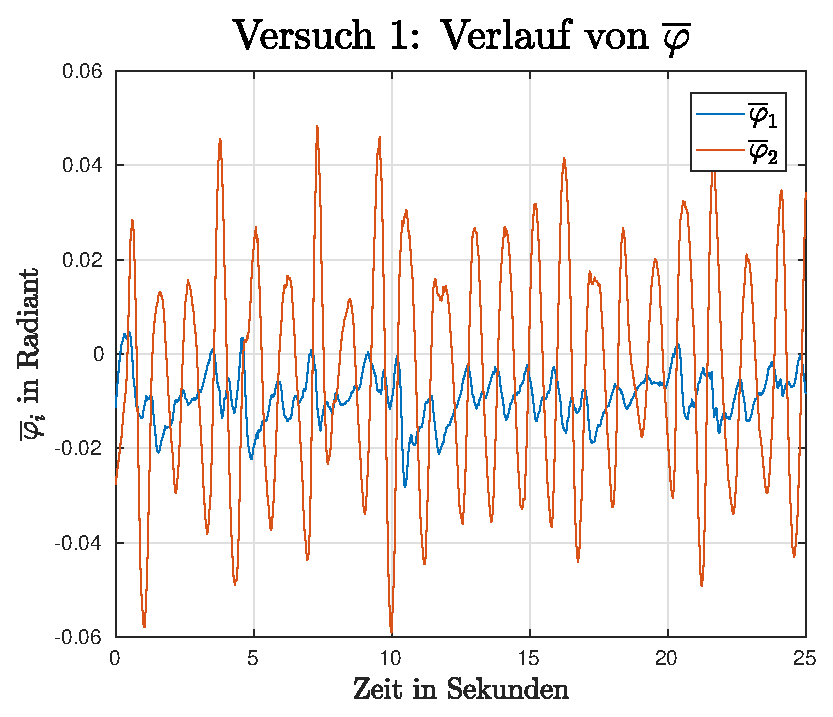
\includegraphics[width=0.45\textwidth]{img/exp1_phi.eps}\hspace{0.7cm}
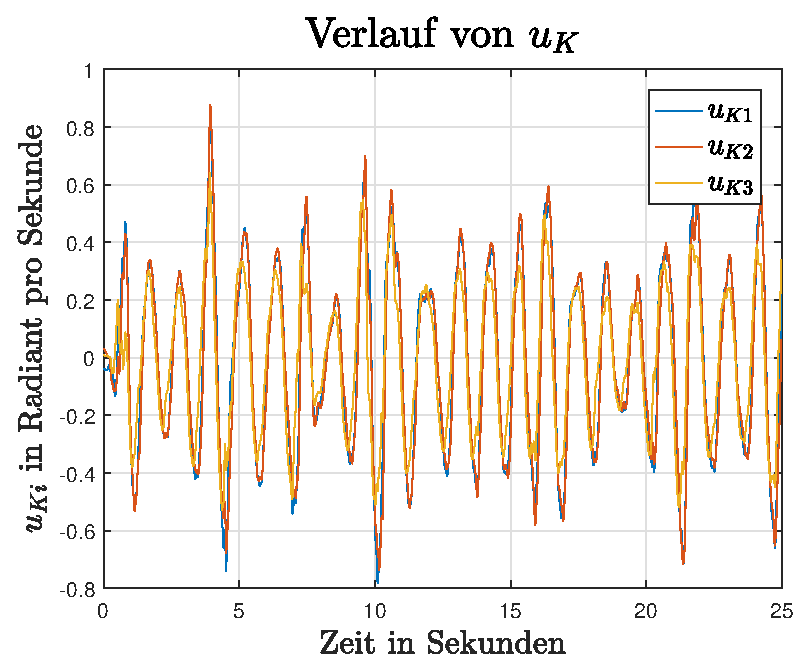
\includegraphics[width=0.45\textwidth]{img/exp1_uk.eps}
\vspace{0.5cm}

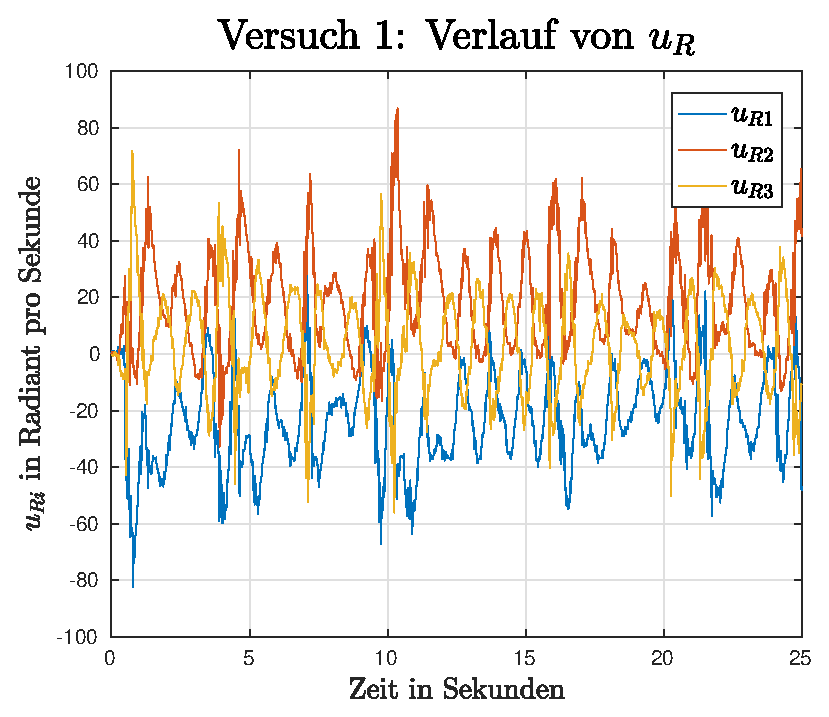
\includegraphics[width=0.45\linewidth]{img/exp1_ur.eps}\hspace{0.7cm}
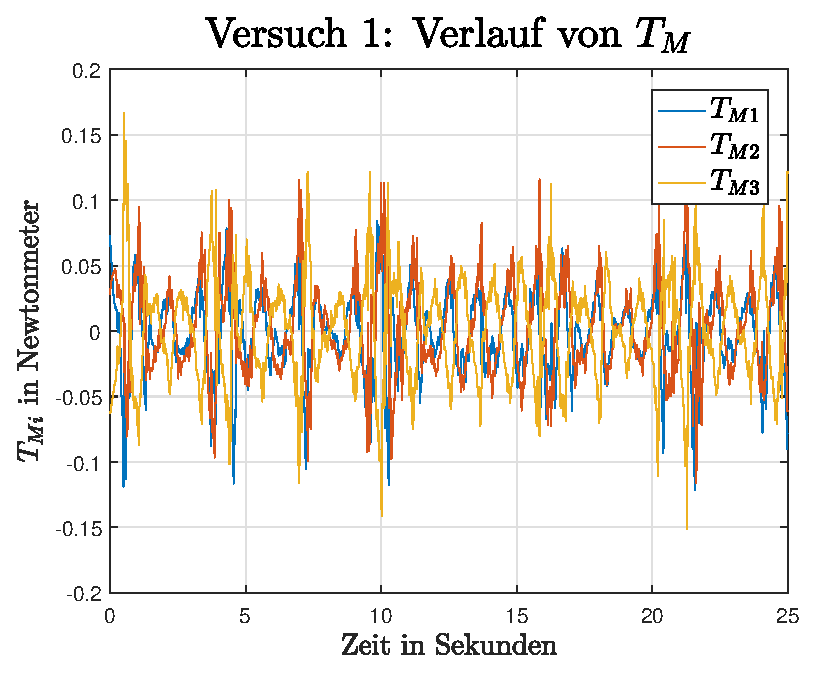
\includegraphics[width=0.45\linewidth]{img/exp1_tm.eps}
\caption{Systemverhalten des geschlossenen Regelkreises}
\end{figure}

Das Experiment zeigt, dass der Regler den Würfel auf einer Ecke stabilisiert. Allerdings ist das System nicht asymptotisch stabil, sondern oszilliert mit einer konstanten Amplitude. Eine mögliche Erklärung für diese Verhalten liegt in der Modellgüte. Um die Direktionalitätsproblematik zu lösen, wurde ein Regler gewählt, welcher die Eigenwerte des geschlossenen Kreises nahe an den Einheitskreis legt. Sind nun die Systemparameter des Modells fehlerbehaftet, ist es möglich, dass die Eigenwerte des realen Regelkreises weiter an den Einheitskreis rücken. In diesem Fall können bereits kleine Anregungen wie z.B. ein in dem Modell nicht erfasstes System- oder Messrauschen zu einer verbleibenden Schwingung führen. Des Weiteren ist der Einfluss der Nichtlinearitäten zu nennen, welche die Auswirkungen der Modellungenauigkeiten zusätzlich beeinflussen können. 

Um die Reglergüte zu verbessern, werden zunächst die Versuchsergebnisse betrachtet. Besonders deutlich ist einerseits die Schwingung des Winkels $\varphi\idx3$. Zudem sind die Signale $u_{\text{K}i}(t)$ nahezu identisch, was einer Rotation des Würfels um seine Raumdiagonale entspricht. Um diese Oszillationen zu dämpfen, werden einzelne Elemente der Reglermatrix schrittweise erhöht und die Veränderung empirisch überprüft. Die veränderten Elemente sind einerseits die Spalte $\bs{K}(:,3)$, welche den Einfluss des Winkels $\varphi\idx3$ auf den Regler wiedergibt, andererseits die Diagonale $\bs{K}(1,4)$, $\bs{K}(2,5)$ und $\bs{K}(3,6)$, welche den Einfluss der Winkelgeschwindigkeit in Richtung der Raumdiagonale wiedergibt. Die Erhöhung dieser Elemente führt dazu, dass die Eigenwerte der zugehörigen Eigenbewegungen näher an den Ursprung gerückt werden. Die folgenden Abbildungen zeigen das Verhalten des geschlossenen Regelkreises, wobei die genannten Elemente der Reglermatrix um den Faktor zwei erhöht wurden.
\begin{figure}[h!]
\centering
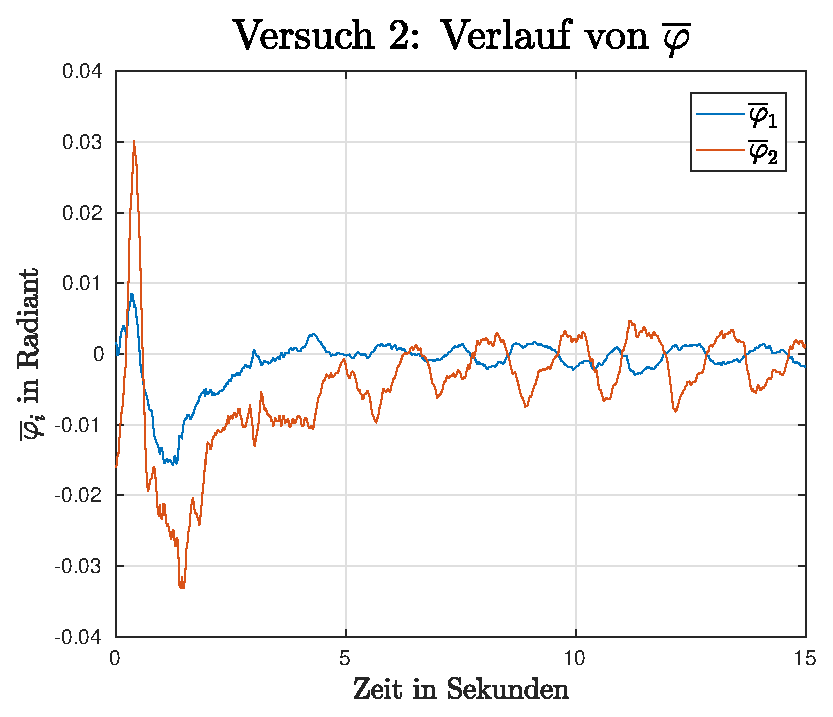
\includegraphics[width=0.45\textwidth]{img/exp2_phi.eps}\hspace{0.7cm}
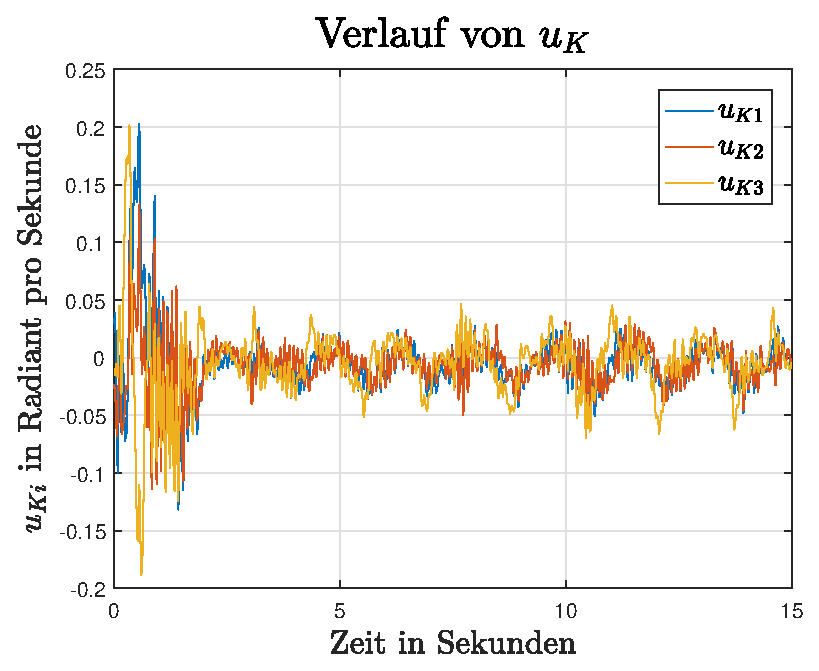
\includegraphics[width=0.45\textwidth]{img/exp2_uk.eps}
\vspace{0.5cm}

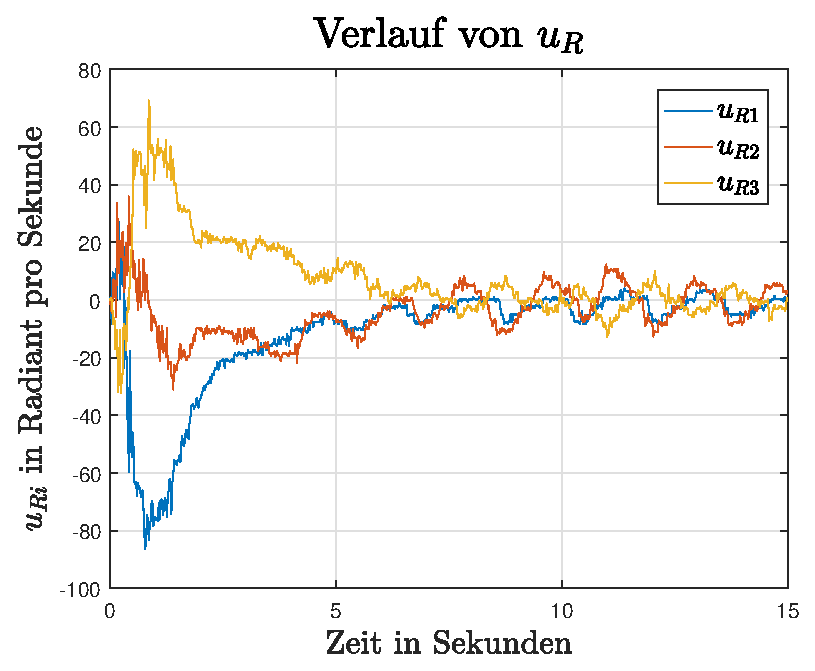
\includegraphics[width=0.45\textwidth]{img/exp2_ur.eps}\hspace{0.7cm}
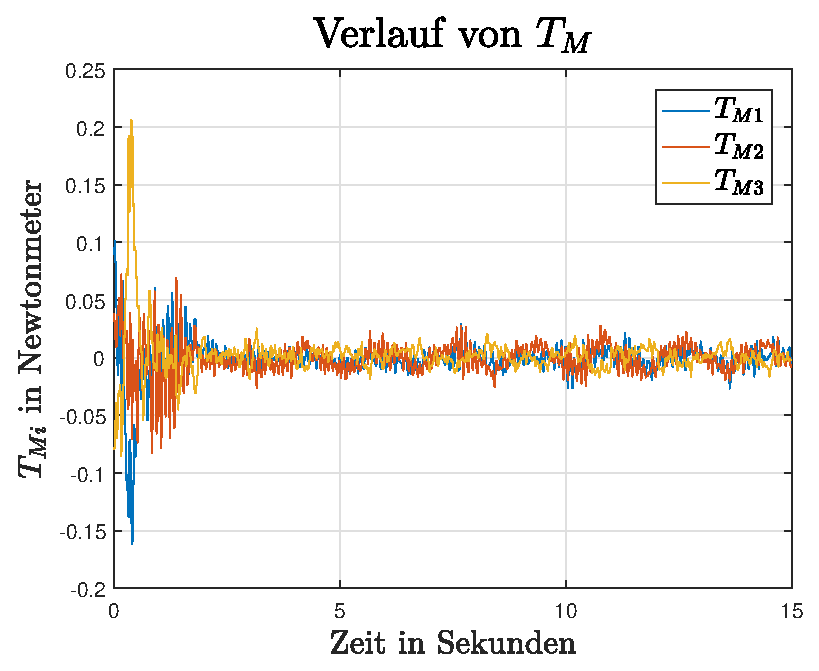
\includegraphics[width=0.45\textwidth]{img/exp2_tm.eps}
\caption{Verhalten des geschlossenen Regelkreises mit angepasstem Regler}
\end{figure}
Daraus geht hervor, dass die Anpassung des Reglers eine deutliche Verbesserung des geschlossenen Regelkreises erzielt. Jedoch ist diese Vorgehensweise kritisch zu beurteilen. Zunächst verbleibt eine Schwingung, welche dem Verhalten im letzten Versuch gleicht. Lediglich die Amplitude der Schwingung wurde durch die Änderung der Reglermatrix reduziert. Außerdem führt der Eingriff in die Reglermatrix dazu, dass die Reglereigenschaften, welche aus dem LQR-Verfahren resultieren, nicht mehr garantiert werden. Insbesondere die Robustheitseigenschaften können verloren gehen. Dies zeigt sich, wenn die Reglerelemente weiter verändert werden, um die verbleibenden Schwingungen zu eliminieren. Derartige Änderungen führen zu einem instabilen Regelkreis.
